\clearpage\section{Computing persistent homology}
\label{sec:computing-persistent-homology}
This section outlines the standard algorithm for computing persistent homology, and some speed-ups that are utilised by Ripser \cite{bauer2021ripser}. Some experiments are conducted to verify speed-ups, and as we add each speed-up we compare it to the previous original algorithm. We introduce the algorithms in the order:

\begin{enumerate}
  \item the standard algorithm (no speed-ups);
  \item sparse matrix representation;
  \item reduction by killing (clearing); and
  \item reducing the cohomology boundary matrix.
\end{enumerate}

Homology will be computed with coefficients in $\mathbb F_2$, given the amenability to a fast algorithm (our algorithms may also be adapted to any field). It is generally agreed that the torsional subgroups of the homology groups with coefficients in some non-divisible group yield no practical information. There are also many challenges to overcome for computing persistent homology over a non-divisible group; for example, our structure theorem for persistence modules does not hold for algebraic structures that are not fields (such as $\mathbb Z$). We pose this as a topic of further research, as not much material exists on its potential uses. Note that the notion of \emph{oriented simplices} does not make much sense over $\mathbb F_2$, as $\overline 1 = \overline{-1}$. 

In the following exposition, we assume homology is calculated up to some fixed dimension $d \in \mathbb N$. Also, for a matrix $M$, we will denote the $i$th column of $M$ by $M_i$. 

We have discussed the existence of a compatible ordering of simplices for a filtered simplicial complex. To make our exposition clearer, we will be considering only \emph{maximal} filtration; that is, filtrations of the form $\{K_i\}_{i=0}^n$ where $K_i = \bigcup_{i=1}^n \{\sigma_i\}$. Thus moving up the filtration by one level corresponds to adding a single simplex. We show how this method can be extended to any filtered simplicial complex.

Let $\mathbb L = \{L_i\}_{i=0}^m$ be any filtered simplicial complex and let $\sigma_1, \ldots, \sigma_n$ be a compatible simplex ordering. We form the maximal filtration $\mathbb K$ by
\[ \mathbb K = \{K_i\}_{i=0}^n, \qquad K_i = \bigcup_{i=1}^n \{\sigma_i\}. \]
We then construct the surjective map
\begin{align*}
  f: \{1, \ldots, n\} & \to \{0, \ldots m\},                 \\
  i                   & \mapsto \min\{j: \sigma_i \in L_j\}.
\end{align*}
This induces a map
\begin{align*}
  f_*: \Pers(H_*(\mathbb K)) & \to \Pers(H_*(\mathbb L)) \\
  (i, j)                     & \mapsto (f(i), f(j))
\end{align*}
(with $f_*(i, \infty) = (f(i), \infty)$) which is a bijection.

\subsection{Standard algorithm}

We first introduce our problem formally.

\begin{problem}[$\mathbb F_2$-PersBarcodes]
  Instance: let $\mathbb K$ be a maximal (finite) filtered simplicial complex. \\
  Question: compute $\Pers(H_*(\mathbb K; \mathbb F_2))$.
\end{problem}

Let $K$ be a finite simplicial complex and $\mathbb K = \{K_i\}_{i=0}^n$ be a maximal filtration of $K$. Let $\sigma_1, \ldots, \sigma_n$ be the (unique) ordering of the simplices of $K$ induced by $\mathbb K$.

We consider the simplicial chain complex of $K$ with coefficients in $\mathbb F_2$: $C(K; \mathbb F_2) = \{(\restr Ki, \partial_i)\}_{i=0}^{\dim K}$. Let $n_i = \left\lvert \restr Ki \right\rvert$. By picking canonical bases for each $\restr Ki$, we may represent $\partial_i$ as a $n_{i-1} \times n_{i}$ matrix with entries in $\mathbb F_2$ for each $i \geq 1$. We combine the boundary maps of each chain group into a single map, $\partial: \bigoplus_{i=0}^{\dim K} C_i \to \bigoplus_{i=0}^{\dim K} C_i$. To do this, we pick our basis as the simplex ordering $\sigma_1, \ldots, \sigma_n$ and let $\partial$ be a $n \times n$ matrix defined by
\[
  \partial[i,j] = \begin{cases}
    1 & \text{if $\sigma_i$ is a face of $\sigma_j$}, \\
    0 & \text{otherwise}.
  \end{cases}
\]
This map agrees with the boundary maps $\partial_i$ of the simplicial chain complex, and $\partial$ is strictly upper triangular. We call $\partial$ the \emph{boundary matrix} of $\mathbb K$.

\begin{figure}
  \centering
  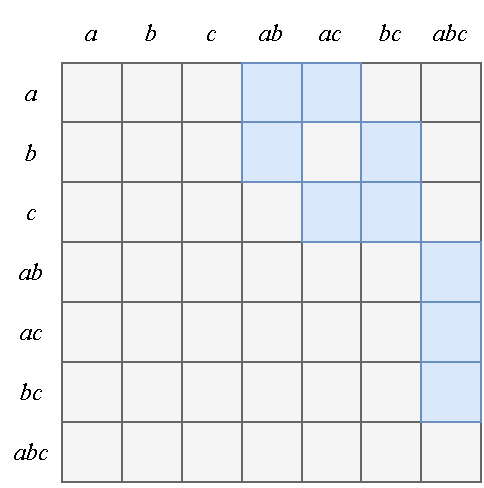
\includegraphics[width=0.5\textwidth]{content/4-comp-top/images/boundary-ex}
  \caption{The boundary matrix for the simplex ordering $(a, b, c, ab, ac, bc, abc)$. A grey cell corresponds to a 0, and a blue cell corresponds to a 1.}
  \label{fig:boundary-ex}
\end{figure}

\begin{example}
  Figure \ref{fig:boundary-ex} is a visualisation the boundary matrix for the simplex ordering $(a, b, c, ab, ac, bc, abc)$.
\end{example}

The prevalent method for solving \textsc{$\mathbb F_2$-PersBarcodes} this problem is matrix reduction (effectively a variant of the Smith normal form algorithm). We let $M \in M_n(\mathbb F_2)$ and define $\low_M(i) = \max\{j: M[i, j] \neq 0\}$; that is, $\low(i)$ is the largest row index of a non-zero entry in column $i$ (we let it take some sentinel value otherwise). A column operation of the form $M_i \gets M_i + M_j$ is called \emph{reducing} if $j < i$ and $\low_M(i) = \low_M(j)$. A matrix is called \emph{reduced} if no more reducing operations can be performed on it. A matrix $R$ is a \emph{reduction} of $M$ if $R$ is reduced and arises from a sequence of reducing operations from $M$.

\begin{lemma}
  \label{lem:reduction-correct}
  Let $K$ be a finite simplicial complex and $\mathbb K = (K_i)_{i=0}^m$ be a filtration of $K$, such that $K_m = K$. Let $\partial$ be the boundary matrix of $\mathbb K$ (with basis some ordering of the simplices compatible with $\mathbb K$) and $R$ a reduction of $\partial$. Then $(i, j) \in \Pers(\mathbb K)$ if and only if
  \begin{enumerate}
    \item $j \neq \infty$ and $\low_R(j) = i$;
    \item $j = \infty$ and $\low^{-1}_R(i) = \varnothing$. 
  \end{enumerate}
\end{lemma}

\begin{proof}
  We can consider the reduction algorithm as a variant of a Smith normal form algorithm (although the reduction matrix is not quite in Smith normal form), and so by the structure we gave the persistence module in Section \ref{ssec:pers_modules} we see that the reduction algorithm indeed gives us the persistent barcodes as above.
\end{proof}

Lemma \ref{lem:reduction-correct} shows us that it is sufficient to find a reduction of the boundary matrix to compute the persistent barcodes. 

Before looking at methods for computing the reduction, we look at how to read off the persistent barcodes. We split $\Pers(H_*(\mathbb K))$ into two sets:
\[ \Pers(H_*(\mathbb K)) = \Pers_0(H_*(\mathbb K)) \cup \Pers_\infty(H_*(\mathbb K))\]
where $\Pers_0(H_*(\mathbb K))$ comprises of the finite intervals $(i,j)$ and $\Pers_\infty(H_*(\mathbb K))$ comprises of the infinite intervals $(i, \infty)$. We can compute $\Pers_0(\mathbb K)$ by iterating over each $j \in \{1, \ldots, n\}$ and computing $\low_\partial(j) = i$, which forms $(i, j) \in \Pers_0(\mathbb K)$. For $\Pers_\infty(H_*(\mathbb K))$, we just note the $i \in \{1, \ldots, n\}$ that does not have a corresponding $j > i$ such that $\low_\partial(j) = i$. The running time of this interpretation depends on the implementation of the $\low$ function; for example, using a hash table gives us a constant time evaluation and $O(n)$ time to update after a column operation, which would give us a constant time interpretation. 

We now introduce the problem of finding the reduction of $\partial$. 

\begin{problem}[$\mathbb F_2$-PersReduction]
  Instance: let $\partial$ be the boundary matrix of some maximal filtered simplicial complex. \\
  Question: compute a reduction $R$ of $\partial$.
\end{problem}

\begin{algorithm}
  \caption{The standard reduction algorithm for \textsc{$\mathbb F_2$-\-Pers\-Reduc\-tion}.}
  \label{alg:std-reduction}
  \begin{algorithmic}[1]
      \Function{Low}{$n \times n$ matrix $R$, $i \in \{1, \ldots, n\}$}
        \State\Return lowest non-zero entry of column $i$
      \EndFunction
      \Function{IsColReduced}{$n \times n$ matrix $R$, $i \in \{1, \ldots, n\}$}
        \State\Return whether there is $i' < i$ such that $\Call{Low}{R, i'} = \Call{Low}{R, i}$
      \EndFunction
      \Function{StdReduction}{$n \times n$ boundary matrix $\partial$}
        \State $R \gets \partial$
        \For{$i \gets 1$ to $n$}
          \While{not \Call{IsColReduced}{$R, i$}}
            \For{$j=1$ to $i$}
              \If{$\Call{Low}{R, i} = \Call{Low}{R, j}$}
                \State add column $j$ to $i$ and break for loop
              \EndIf
            \EndFor
          \EndWhile
        \EndFor
        \State\Return $R$
      \EndFunction
  \end{algorithmic}
\end{algorithm}

Algorithm \ref{alg:std-reduction} is the standard reduction algorithm for persistent homology, first introduced by \textcite{edelsbrunner2000topological}. We will refer to this algorithm as \textsc{S}.

The running time of Algorithm \ref{alg:std-reduction} is $O(n^3)$ as
\begin{enumerate}
  \item adding a column to another column runs in $O(n)$ time; and
  \item calling the function $\textsc{Low}$ can be achieve in $O(1)$ time using a hash table, this hash table can be updated in $O(n)$ for each column operation.
\end{enumerate}

We are clear on the correctness of such a reduction, if the algorithm terminates then it is clear we meet the requirements of $R$ being a reduction. But we must prove that Algorithm \ref{alg:std-reduction} terminates. On to the main loop (line \texttt{9} onwards), we first claim that this terminates. Although not immediately obvious, we assert that $\textsc{IsColReduced}(i)$ will evaluate true by repeating \texttt{11} to \texttt{15}. Trivially, $\textsc{IsColReduced}(1)$ is always true. We now let $i > 1$ and assume that $\textsc{IsColReduced}(j)$ is true for each $j \in \{1, \ldots i\}$. As $\textsc{IsColReduced}(i)$ is false, there is $i_1 < i$ such that $\textsc{Low}(i_1) = \textsc{Low}(i)$. So we add the $i_1$th column to the $i$th column, making the new value of $\textsc{Low}(i)$ strictly less than $\textsc{Low}(i_1)$ (as, by definition, every entry below $\textsc{Low}(i_1)$ is zero). To appreciate this, we recall that we are in $\mathbb F_2$. If $\textsc{IsColReduced}(i)$ is true, we are done; otherwise, there is $i_2 < i$ such that $\textsc{Low}(i_2) = \textsc{Low}(i) < \textsc{Low}(i_1)$. Again, we perform the appropriate column operation. We continue this operation, and as there are only a finite number of rows (that is, a finite number of unique values for \textsc{Low}), then we must reach a point at which $\textsc{IsColReduced}(i)$ is false. The final conclusion is clear by induction. 


% First, we learn to read the ranks of the homology groups of $K$. Let $R \in M_m(\mathbb F_2)$ be the resulting matrix from running the standard algorithm described above on $\partial$. Define
% \begin{align*}
%   \operatorname{zeros}_p(R) & = \left\{
%   i: \text{column $i$ in $R$ is zero and $\dim\sigma_i=p$}
%   \right\},                             \\
%   \operatorname{lows}_p(R)  & = \left\{
%   i: \text{$\operatorname{low}(j) = i$ for some $j$ and $\dim\sigma_i=p$}
%   \right\}.
% \end{align*}
% If $K_i = \{\sigma_j\}_{j=1}^i$, we claim that $\operatorname{zeros}_p(R) - \operatorname{lows}_p(R) = \beta_p$, which can be seen by observing that $\operatorname{zeros}_p(R)$ is the rank of the $p$-cycles, and $\operatorname{lows}_p(R)$ is the rank of the $p$-boundaries.

% Next, we move to persistent homology. Let $f: K \to \R$ be defined on our simplicial complex as in the last section which induces our filtration, with associated sequence $\{a_i\}_{i=0}^m$. If $K_i = \{\sigma_j\}_{j=1}^i$ then $(a_i, a_j) \in \dgm_p(f)$ if and only if $i = \operatorname{low}(j)$ and $\dim\sigma_i = p$. Now we assume otherwise, so there is a step in the filtration in which more than one simplex is added. We simply construct the filtration $\{K_i'\}_{i=0}^m$ such that $K_i' =  \{\sigma_j\}_{j=1}^i$ and let $k': \Z_{\geq 0} \to \Z_{\geq 0}$ be the sequence such that $K_i = K'_{k'(i)}$ for all $i$. Now define $k: \Z_{\geq 0} \to \Z_{\geq 0}$ as $i \mapsto \min\{i': k(i') \geq i \}$. This is a mapping between our filtration and a filtration which only adds one simplex at a time when we move up. Let $(i, j)$ be the indices of some point in the $p$th persistence diagram for $K'$. Then $(a_{k(i)}, a_{k(j)}) \in \dgm_p(f)$

\subsection{Spare matrix representation}

The first speed-up we look at utilises the \emph{sparseness} of the boundary matrix. To motivate, we consider a triangulation of $S^n$. Let $K$ be a simplicial complex consisting of the proper faces of some $(n+1)$-simplex and $\mathbb K$ be a maximal filtration of $K$ where we add the $0$-simplices, then the $1$-simplices, and so on. We note that there is $2^{n+2} - 2$ simplices. For $n = 2$, Figure \ref{fig:sparse-matrix-ex} shows a boundary matrix for $\mathbb K$ (recall that we are in $\mathbb F_2$, a blue square represents a 1 and a grey square represents a 0).

\begin{figure}
  \centering
  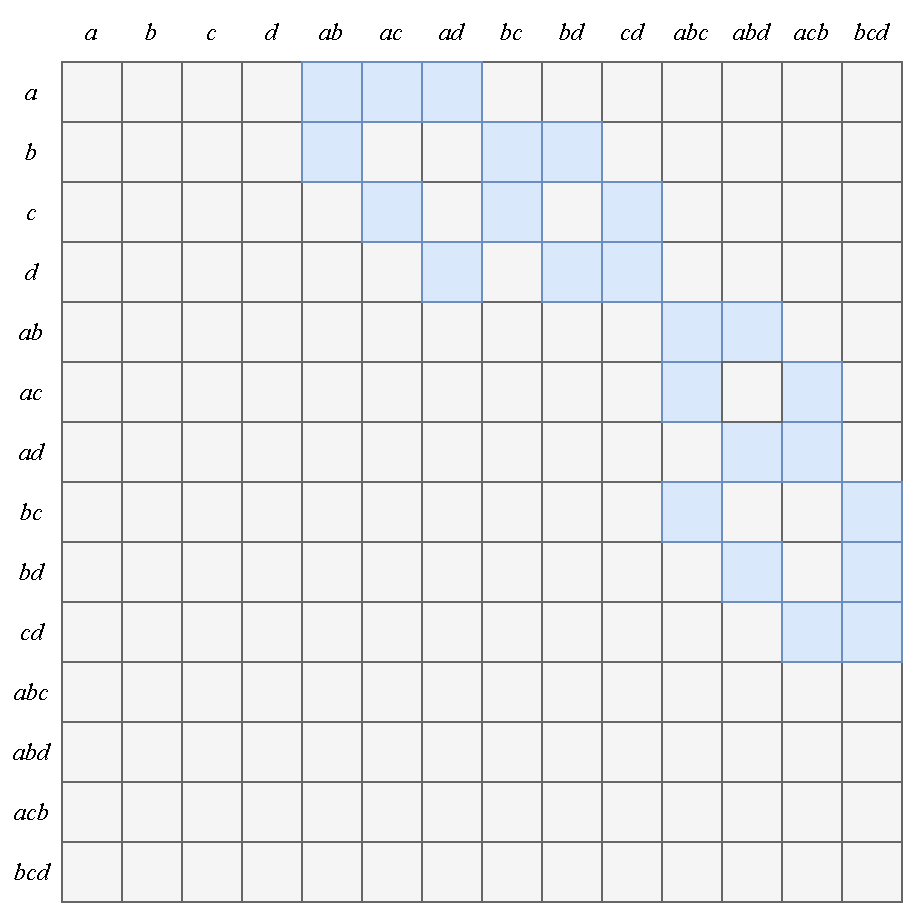
\includegraphics[width=0.7\textwidth]{content/4-comp-top/images/sparse-matrix-ex}
  \caption{A sparse boundary matrix for a filtration of a triangulation of $S^2$. A grey square represents a $0$ entry in the matrix, and a blue square represents a $1$.}
  \label{fig:sparse-matrix-ex}
\end{figure}

Figure \ref{fig:sparse-matrix-ex} shows a \emph{sparse matrix}; most of the entries are zero. Boundary matrices for general filtered simplicial complex are also sparse. Although most entries are 0, we are still storing each one: the standard algorithm stores a value for each $(i, j) \in (1, \ldots, n)^2$. There are many efficient methods for storing a sparse matrix, and most make use of assuming all entries are zero, then provide additional information for the non-zero entries. We will provide one such way of doing this, which is suited to our problem. 

\begin{figure}
  \centering
  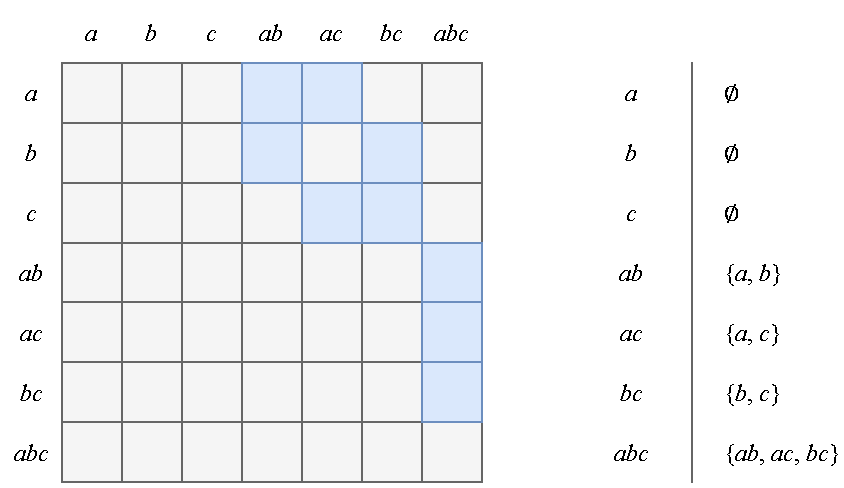
\includegraphics[width=0.9\textwidth]{content/4-comp-top/images/sparse-representation-ex}  
  \caption{On the left, the boundary matrix for the simplex ordering $(a, b, c, ab, ac, bc, abc)$. On the right, the sparse matrix representation. A grey square represents a $0$ entry in the matrix, and a blue square represents a $1$.}
  \label{fig:sparse-representation-ex}
\end{figure}

Let $A \in M_n(\mathbb F_2)$ be a matrix. For each column $j \in \{1, \ldots n\}$, we store a set (hash table), denoted $S_j$, such that $i \in S_j$ if and only if $A[i,j] = 1$. This allows constant time for many elementary operations (such as membership queries, insertion, and deletion) and constant space. Figure \ref{fig:sparse-representation-ex} shows an example of this representation. We further comment on the running time of operations with this data structure, specific to the reduction algorithm. For $i \in \{1, \ldots, n\}$, denote the number of non-zero entries in column $i$ by $m_i$, and we have $O(m_i) = O(d)$.

\begin{enumerate}
  \item Column operations: let $i, j \in \{1, \ldots, n\}$ . Then the time to add column $j$ to $i$ is $O(m_i + m_j)$. Given that we typically fix the dimensions to compute homology to, we can take this as constant (or as $O(d)$ for maximum dimension $d$).
  \item Retrieve the last non-zero entry in column: let $i \in \{1, \ldots, n\}$. Finding the last non-zero entry in $i$ is $O(m_i)$.
\end{enumerate}

As we are just modifying the underlying data structure, the algorithm does not change significantly and thus will not be repeated here. We refer to the standard algorithm with sparse matrix representation as \textsc{SS}. 

This analysis provides a convincing argument the effectiveness of this speed-up. To quantify this, an experiment was conducted in which measured the running time for both loading (that is, taking a filtration and computing its boundary matrix) and the matrix reduction for the standard triangulation of $S^n$ for $n \in \{1, \ldots, 9\}$. The running times can be seen in Figure \ref{fig:speedups-1v2-compute} and the loading running times can be seen in Figure \ref{fig:speedups-1v2-load}.

\begin{figure}
  \makebox[\textwidth][c]{
    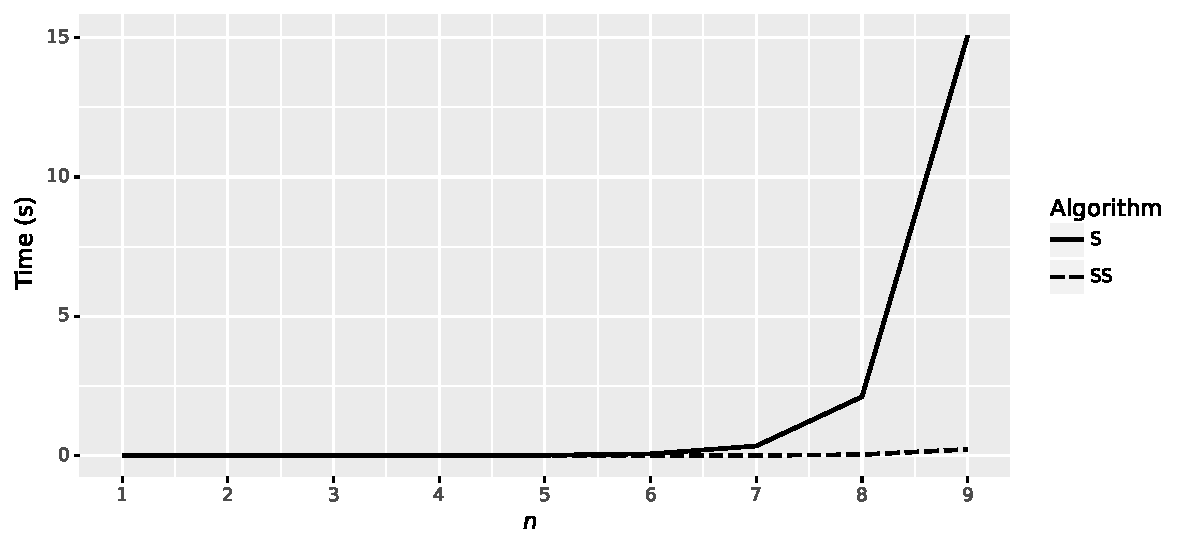
\includegraphics[width=1.2\textwidth]{content/4-comp-top/images/2-1v2-compute}
  }
  \caption{A plot of the running time of the \textsc{SS} algorithm versus the \textsc{S} algorithm for filtrations of triangulations of $S^n$.}
  \label{fig:speedups-1v2-compute}
\end{figure}

\begin{figure}
  \makebox[\textwidth][c]{
    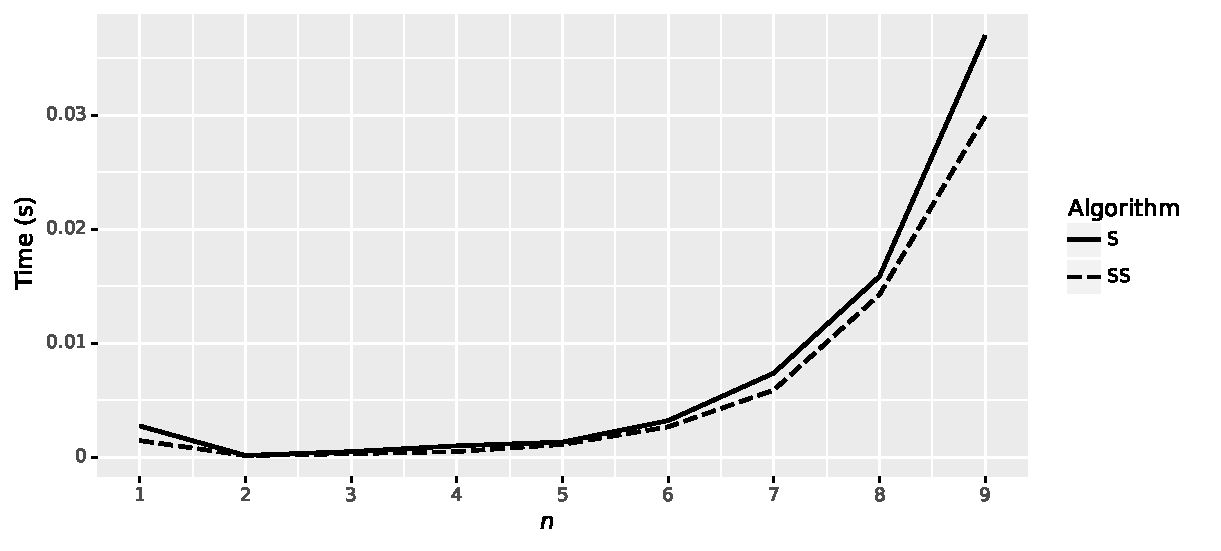
\includegraphics[width=1.2\textwidth]{content/4-comp-top/images/2-1v2-load}
  }
  \caption{A plot of the running time of the construction of the boundary matrix (loading time) using the standard matrix representation versus the sparse matrix representation, for filtrations of triangulations of $S^n$.}
  \label{fig:speedups-1v2-load}
\end{figure}

From this experiment, we see that the sparse matrix representation significantly decreases the time taken by the reduction; however, it does not decrease the loading time. This is to be expected as we still need to iterate over every the facets of every simplex; however, we note that this input serves as a worse case for loading time, so we would expect a large running time for loading compared to other inputs.

Another experiment was conducted using a Vietoris-Rips complex (with $\hat\varepsilon = 0.01$) constructed from point-cloud data sampled from a noisy unit circle (radius fluctuation $0.1$). Each algorithm was executed on a complex constructed from $n$ points, where $n \in \{100, 200, \ldots, 1500\}$. Figure \ref{fig:speedups-1v2-circ-compute} shows the running time of both of these algorithms, and it is clear that the sparse representation is still significantly faster.

\begin{figure}
  \makebox[\textwidth][c]{
    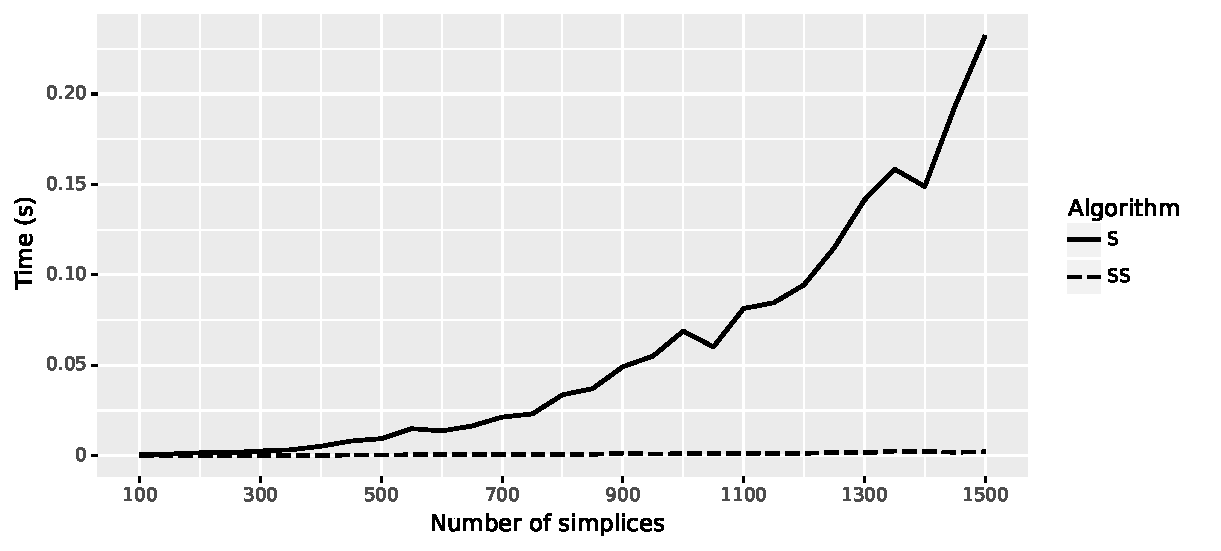
\includegraphics[width=1.2\textwidth]{content/4-comp-top/images/2-1v2-circ-compute}
  }
  \caption{A plot of the running time of the \textsc{SS} algorithm versus the \textsc{S} algorithm for Vietoris-Rips complexes constructed from noisy unit circle data.}
  \label{fig:speedups-1v2-circ-compute}
\end{figure}

We note that there are other data structure choices that could be made instead of hash tables. For example, for each column we may instead store some sorted data structure. If we use a list sorted by index then we can retrieve the lowest non-zero entry in constant time, but we have $O(n)$ time for insertion, deletion, and membership queries. Binary search trees could also be used, which would allow us to find the lowest non-zero entry in $O(\log n)$ average time, as well as $O(\log n)$ average time for insertion, deletion, and membership queries. Utilising self-balancing tree structures (such as B-trees), the worst-case time can also be brought down to $O(\log n)$.

We highlight the use of various data structures for storing a boundary matrix to be a topic of further research.

\subsection{Reduction by killing}

Reduction by killing allows us to \emph{clear} (set to $\bm 0$) certain columns throughout the reduction process, allowing us to avoid unnecessary column operations that would lead the column to being zero anyway. This technique was first introduced by \textcite{chen2011persistent}.

We recall that persistent homology aims to track the changes to the homology groups of a chain complex as we move through a filtration. We now formalise how simplices may change the homology groups.

\begin{definition}[Positive and negative simplices]
  Let $\mathbb K = \{K_i\}_{i=0}^n$ be a maximal filtered simplicial complex of a simplicial complex $K$ with induced simplex ordering $\sigma_1, \ldots, \sigma_n$. Let $\iota_i: K_i \xhookrightarrow{} K_{i+1}$ be the inclusion map and $\overline\iota_i: H_*(K_i) \to H_*(K_{i+1})$ the induced map on homology. 
  \begin{enumerate}
    \item $\sigma_i \in K$ is said to be a \emph{positive simplex} if its addition creates a homology class. That is, for all $[c] \in H_*(K_{i-1})$ we have $\overline\iota_{i-1}([c]) \neq [\sigma_i] \in H_*(K_i)$.
    \item $\sigma_i \in K$ is said to be a \emph{negative simplex} if it its addition destroys a homology class. That is, there is $[c], [c'] \in H_*(K_{i-1})$ with $[c] \neq [c']$ such that $\overline\iota_{i-1}([c]) = \overline\iota_{i-1}([c']) = [\sigma] \in H_*(K_i)$.
  \end{enumerate} 
\end{definition}

We can pair each negative simplex $\sigma_j \in K$ with the positive simplex $\sigma_i \in K$ ($i < j$) that created the class that $\sigma_j$ destroys. We call $(i, j)$ (or $(\sigma_i, \sigma_j)$) a \emph{persistence pair}, and $j - i$ its \emph{index persistence}. It is clear (from the definition of homology) that for a persistence pair $(\sigma_i, \sigma_j)$, we have $\dim\sigma_i = \dim\sigma_j - 1$. 

\begin{corollary}\label{lem:positive-or-negative-simplices}
  Let $\mathbb K = \{K_i\}_{i=0}^n$ be a maximal filtered simplicial complex of a simplicial complex $K$. Then every simplex $\sigma \in K$ is either \emph{positive} or \emph{negative}.
\end{corollary}

This is a direct consequence of Lemma \ref{lem:reduction-correct}.

Note that, although each simplex either creates or destroys a homology class, not every simplex belongs to a persistence pair as described above. In particular, certain simplices create homology classes that persist through to the final complex, $K_n = K$. Such (positive) simplices are called \emph{essential simplices}.

The following is the key observation for reduction by killing.

\begin{lemma} \label{lem:clearing-lemma}
  Let $\mathbb K = \{K_i\}_{i=0}^n$ be a maximal filtered simplicial complex of a simplicial complex $K$ with induced simplex ordering $\sigma_1, \ldots, \sigma_n$, let $R$ be the reduction of the boundary matrix of $\mathbb K$ (with respect to our ordering), and let $(i, j) \in \Pers(H_*(\mathbb K))$. Then $R_i = \bm 0$. 
\end{lemma}

\begin{proof}
  As $(i, j) \in \Pers(H_*(\mathbb K))$, $\low_R(j) = i$. Suppose $R_i \neq 0$, then $\low_R(i) = i'$ for some $i \in \{1, \ldots, n\}$. But then $(\sigma_{i'}, \sigma_i)$ is a persistence pair, contradicting Corollary \ref{lem:positive-or-negative-simplices}.
\end{proof}

So if we discover a negative simplex $\sigma$, we can clear the column corresponding to the simplex whose homology class $\sigma$ kills. However, the standard algorithm \textsc{S} starts at the left side of the boundary matrix and moves to the right, so we will always discover positive simplices first. Thus we do not save any column operations. 

To take advantage of Lemma \ref{lem:clearing-lemma}, we instead reduce the boundary matrix right-to-left. We first clear the $d = \dim K$ simplices (from left-to-right), then the $(d-1)$-simplices, and so on. 

Algorithm \ref{alg:reduction-by-killing} shows the modified algorithm, and we denote this speed-up with the sparse matrix representation on top of the standard algorithms as \textsc{SSR}.

\begin{algorithm}
  \caption{The reduction by killing (\textsc{SSR}) algorithm for \textsc{$\mathbb F_2$-\-Pers\-Reduc\-tion}.}
  \label{alg:reduction-by-killing}
  \begin{algorithmic}[1]
      \Function{StdReduction}{$n \times n$ boundary matrix $\partial$}
        \State $R \gets \partial$
        \For{$k \gets d$ to $1$}
          \For{$i \gets 1$ to $n$}
            \If{simplex $i$ does not have dimension $k$}
              \State continue to next simplex
            \EndIf
            \While{not \Call{IsColReduced}{$R, i$}}
              \For{$j=1$ to $i$}
                \If{$\Call{Low}{R, i} = \Call{Low}{R, j}$}
                  \State add column $j$ to $i$ and break for loop
                \EndIf
              \EndFor
            \EndWhile
            \If{$R_j \neq \bm 0$}
              \State clear column $\low(R, j)$
            \EndIf
          \EndFor
        \EndFor
        \State\Return $R$
      \EndFunction
  \end{algorithmic}
\end{algorithm}

An experiment was conducted comparing \textsc{SS} and \textsc{SSR}. A Vietoris-Rips filtration was constructed from a sample of 1000 points from the noisy unit circle (radius fluctuation $\pm 0.05$). We run both algorithms from $\varepsilon = 0.01$ to $\varepsilon = 0.06$. Figure \ref{fig:speedups-2v3-compute} shows the result of this experiment.

\begin{figure}
  \makebox[\textwidth][c]{
    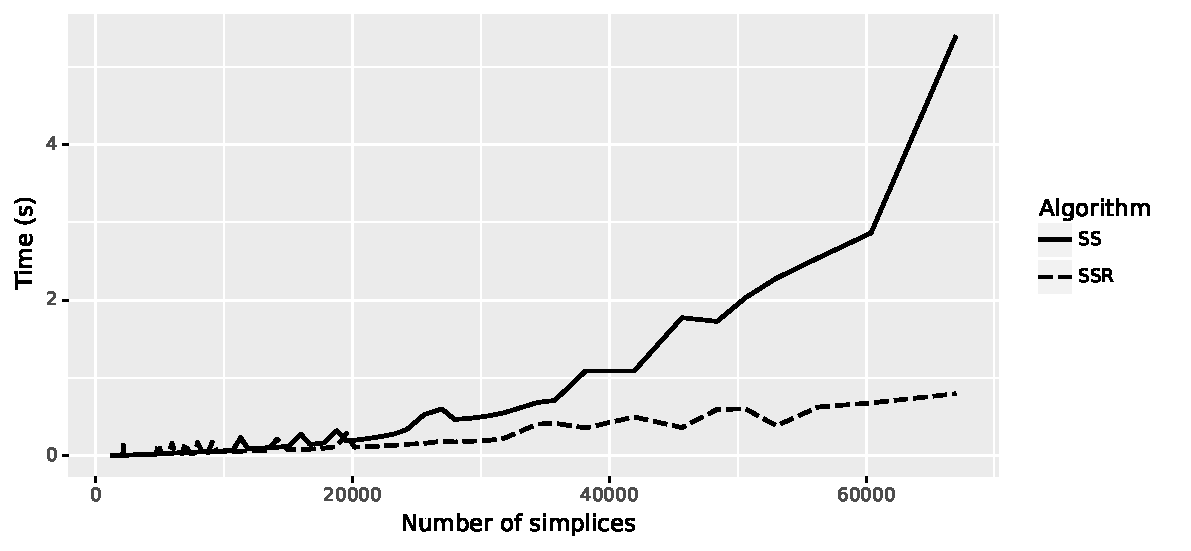
\includegraphics[width=1.2\textwidth]{content/4-comp-top/images/2-2v3-circ-compute}
  }
  \caption{A plot of the running time of \textsc{SS} and \textsc{SSR} algorithms on a Vietoris-Rips complex constructed from a noisy unit circle.}
  \label{fig:speedups-2v3-compute}
\end{figure}

It can be seen that \textsc{SSR} significantly decreases computation time as the number of simplices increase, due to the reduction of column operations. 

\subsection{Reducing the coboundary matrix}

The reduction by killing method (clearing) was found to be utilised to a much greater degree when using the cohomology (instead of the homology) of Vietoris-Rips filtrations. \textcite{de2011dualities} first published this cohomology algorithm; however, it compares the use of cohomology to the standard algorithm without clearing and thus his results may artificially bloat the effectiveness of this speed-up.

There are two main observations to understand this speed-up:
\begin{enumerate}
  \item the persistent barcodes from homology and cohomology are identical; and
  \item computing persistent barcodes on cohomology allows for more clearing.
\end{enumerate}

We have already seen that the persistent barcodes for homology and cohomology coincide (see Lemma \ref{lem:hom-cohom-barcodes-equiv}).

Let $\mathbb K = \{K_i\}_{i=0}^n$ be a maximal filtered simplicial complex and let $\sigma_1, \ldots, \sigma_n$ be the induced simplex ordering. The \emph{coboundary matrix} of $\mathbb K$ is defined by
\[ 
  \delta[i, j] = 
  \begin{cases}
    1 & \text{if $\sigma_{n+1-i}$ is a cofacet of $\sigma_{n+1-j}$}, \\
    0 & \text{otherwise}.
  \end{cases} 
\]
$\delta$ is simply the \emph{anti-transpose} (flip over the anti-diagonal) of the boundary matrix $\partial$, and we can construct it in the same time. We note that the basis for this matrix are the \emph{cochains} of the simplicial cochain complex, and thus mapping between the barcodes from persistent cohomology and persistent homology is just reversing the ordering of our basis (and mapping barcodes of the form $(\infty, i)$ to the form $(j, \infty)$ appropriately).

We now argue that cohomology allows for more clearing. In fact, this is not true for the general case. It is the properties of the Vietoris-Rips filtration that allow for more clearing. 

The clearing optimisation (\textsc{SSR}) sets a column $R_i$ to $\bm 0$ if $i$ is the pivot index of another column $R_j$. In terms of persistent barcodes, $R_i$ is a \emph{birth column} and $R_j$ is the \emph{death column}. It has already been noted that $\dim(\sigma_i) = \dim(\sigma_j) - 1$. Thus to clear the column of a $k$-simplex, we must reduce the column of a $(k+1)$-simplex. Conversely, in cohomology, clearing the column a $k$-simplex requires the reduction of the column of a $(k-1)$-simplex. Thus, as 

For Vietoris-Rips filtrations, the degree we calculate persistent homology to is often small, and there are often many more $(d+1)$-simplices than simplices of lower dimension. In homology, clearing is not available for the $(d+1)$-simplices. However, in cohomology, clearing is not available for the $0$-simplices. As there are (often) more $(d+1)$-simplices then $0$-simplices, cohomology allows for more clearing for Vietoris-Rips filtrations.

We refer to the algorithm utilising sparse matrix representation, reduction by killing, and the cohomology boundary matrix as \textsc{SSRCoh}. 

An experiment was conducted comparing \textsc{SSR} and \textsc{SSRCoh}. A Vietoris-Rips filtration was constructed from a sample of 1000 points from the noisy unit circle (radius fluctuation $\pm 0.05$), as in the last experiment. We run both algorithms from $\varepsilon = 0.01$ to $\varepsilon = 0.06$. Figure \ref{fig:speedsup-3v4} shows the result of this experiment, and empirically verifies our predicted speed-up.

\begin{figure}
  \makebox[\textwidth][c]{
  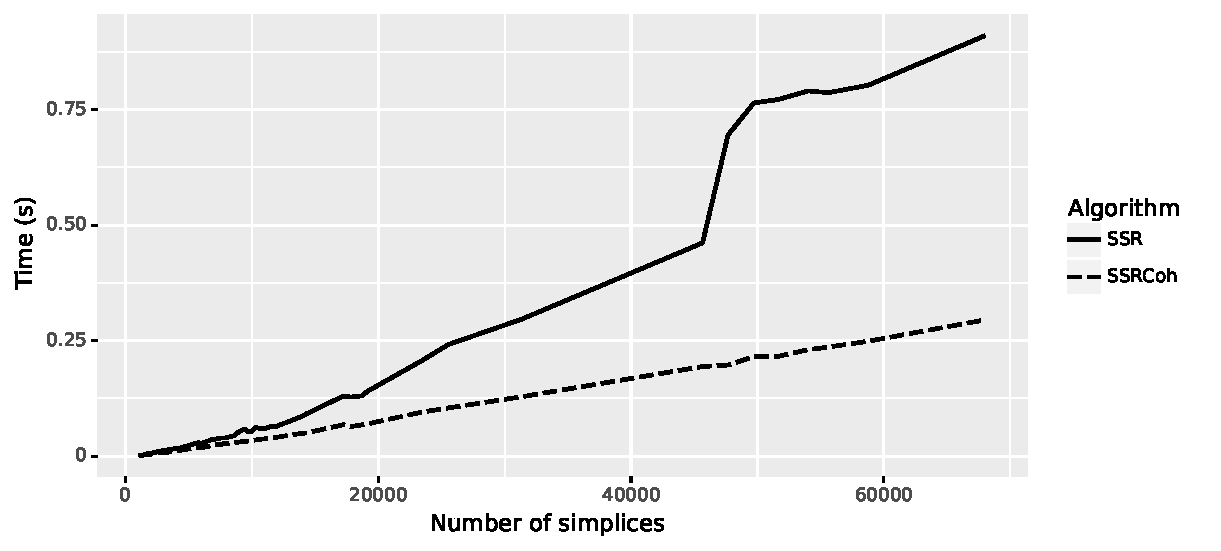
\includegraphics[width=1.2\textwidth]{content/4-comp-top/images/2-3v4-circ-compute}
  }
  \caption{A plot of the running time of \textsc{SSR} and \textsc{SSRCoh} algorithms on a Vietoris-Rips complex constructed from a noisy unit circle.}
  \label{fig:speedsup-3v4}
\end{figure}
